\documentclass{poly}
\usepackage{main}

\title{Chapitre 8 : Étude de fonctions}
\author{Seconde}
\date{}

\begin{document}
\maketitle
\section{Fonctions croissantes et décroissantes}
\begin{definition}
Soit $f$ une fonction à valeurs réelles, et $I$ un intervalle sur lequel $f$ est définie.
\begin{itemize}
\item On dit que $f$ est \textbf{croissante sur $I$}, si pour tout $x < y \in I$, on a $f(x) \leq f(y)$.  
\item On dit que $f$ est \textbf{strictement croissante sur $I$}, si pour tout $x < y \in I$, on a $f(x) < f(y)$.  
\item On dit que $f$ est \textbf{décroissante sur $I$}, si pour tout $x < y \in I$, on a $f(x) \geq f(y)$.  
\item On dit que $f$ est \textbf{strictement décroissante sur $I$}, si pour tout $x < y \in I$, on a $f(x) > f(y)$.
\item On dit que $f$ est \textbf{constante sur $I$}, si pour tout $x < y \in I$, on a $f(x) = f(y)$
\end{itemize}
\end{definition}
\begin{remark}
\hfill
\begin{itemize}
\item Si l'intervalle $I$ est clair suivant le contexte, alors on peut dire qu'une fonction est croissante ou décroissante sans préciser l'intervalle $I$.
\item On dit qu'une fonction croissante (ou strictement croissante) \textbf{conserve l'ordre}, tandis qu'une fonction décroissante (ou strictement décroissante) \textbf{inverse l'ordre}.
\end{itemize}
\end{remark}
\begin{definition}
Soit $f$ une fonction à valeurs réelles, et $I$ un intervalle sur lequel $f$ est définie. 
\begin{itemize}
\item On dit que $f$ est \textbf{monotone sur $I$} si $f$ est croissante sur $I$ ou si $f$ est décroissante sur $I$.
\item On dit que $f$ est \textbf{strictement monotone sur $I$} si $f$ est strictement croissante sur $I$ ou si $f$ est strictement décroissante sur $I$.
\end{itemize}
\end{definition}
\begin{remark}
Pour déterminer qu'une fonction n'est pas monotone sur un intervalle $I$, il suffit de trouver trois réels $x < y < z \in I$ tels que $f(x)$, $f(y)$ et $f(z)$ ne soient pas dans le même ordre (Ni $f(x) \leq f(y) \leq f(z)$, ni $f(x) \geq f(y) \geq f(z)$). 
\end{remark}
\begin{example}
Utiliser le repère ci-dessous pour dessiner la courbe représentative d'une fonction \textbf{non monotone} sur $[-5;5]$.
\begin{center}
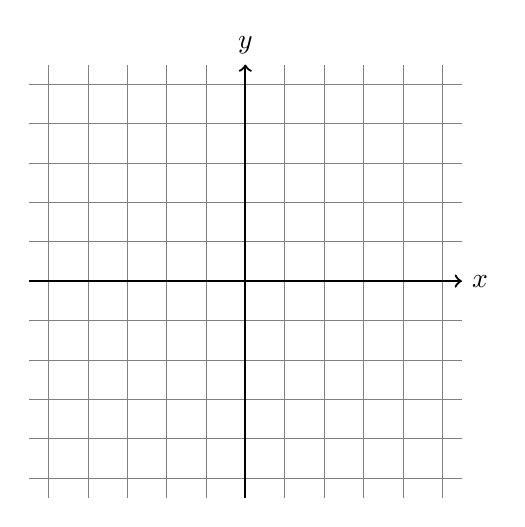
\begin{tikzpicture}
\draw[help lines] (-2.75,-2.75) grid[step=0.5] (2.75,2.75);
\draw[->,thick] (-2.75,0) -- (2.75,0) node[right] {$x$}; 
\draw[->,thick] (0,-2.75) -- (0,2.75) node[above] {$y$};
\end{tikzpicture}
\end{center}
\end{example}
\newpage
\section{Tableaux de variation}
Soient $f$ et $g$ deux fonctions définies sur $[-5;5]$ dont les courbes représentatives sont données ci-contre.
\vspace*{0.5cm}

\begin{minipage}{0.45\textwidth}
\begin{center}
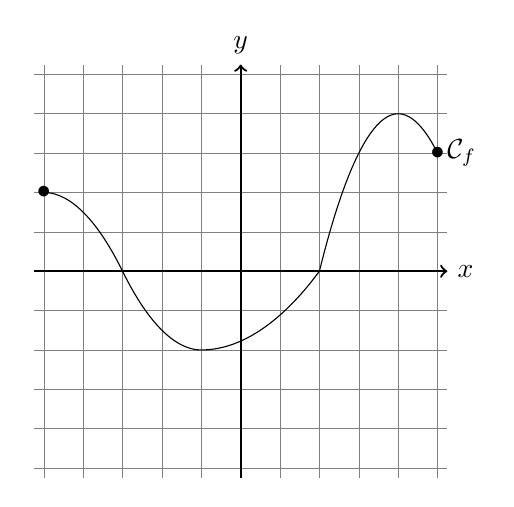
\begin{tikzpicture}[scale=0.5]
\draw[help lines] (-5.25,-5.25) grid (5.25,5.25);
\draw[->,thick] (-5.25,0) -- (5.25,0) node[right] {$x$}; 
\draw[->,thick] (0,-5.25) -- (0,5.25) node[above] {$y$};
\draw (-5,2) node {$\bullet$};
\draw (5,3) node {$\bullet$} node[right] {$\mathcal{C}_f$};
\draw (-5,2) parabola (-3,0);
\draw (-3,0) parabola[bend at end] (-1,-2);
\draw (-1,-2) parabola (2,0);
\draw (2,0) parabola bend (4,4) (5,3);
\end{tikzpicture}
\end{center}
\end{minipage}
\hfill\vline\hfill
\begin{minipage}{0.45\textwidth}
\begin{center}
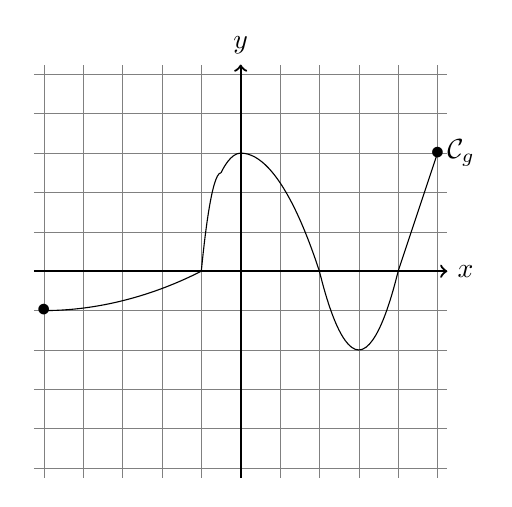
\begin{tikzpicture}[scale=0.5]
\draw[help lines] (-5.25,-5.25) grid (5.25,5.25);
\draw[->,thick] (-5.25,0) -- (5.25,0) node[right] {$x$}; 
\draw[->,thick] (0,-5.25) -- (0,5.25) node[above] {$y$};
\draw (-5,-1) node {$\bullet$};
\draw (5,3) node {$\bullet$} node[right] {$\mathcal{C}_g$};
\draw (-5,-1) parabola (-1,0);
\draw (-1,0) parabola[bend at end] (-0.5,2.5);
\draw (-0.5,2.5) parabola bend (0,3) (2,0);
\draw (2,0) parabola bend (3,-2) (4,0);
\draw (4,0) -- (5,3);
\end{tikzpicture}
\end{center}
\end{minipage}

\vspace*{0.5cm}
\begin{definition}
Le tableau de variation répertorie les plus grand intervalles sur lesquels les fonctions sont monotones. 
\end{definition}
\begin{example}
\hfill

\vspace*{0.2cm}
\begin{minipage}{0.45\textwidth}
\begin{tikzpicture}
\tkzTabInit[espcl=1.5]{$x$ / 1, Variations de $f$ / 2}{$-5$,$-1$,$4$,$5$};
\tkzTabVar{+/$2$,-/$-2$,+/$4$, -/$3$};
\end{tikzpicture}
\end{minipage}
\hfill\vline\hfill
\begin{minipage}{0.45\textwidth}
\begin{tikzpicture}
\tkzTabInit[espcl=1.5]{$x$ / 1, Variations de $g$ / 2}{$-5$,,, $5$}; 
\end{tikzpicture}
\end{minipage}
\end{example}

\newpage
\section{Fonctions de Références}
\subsection{Fonctions carré, racine carrée, inverse et cube}
\begin{minipage}{0.4\textwidth}
\begin{center}
\textbf{Fonction carrée\\$\function{f}{\R}{\R}{x}{x^2}$}
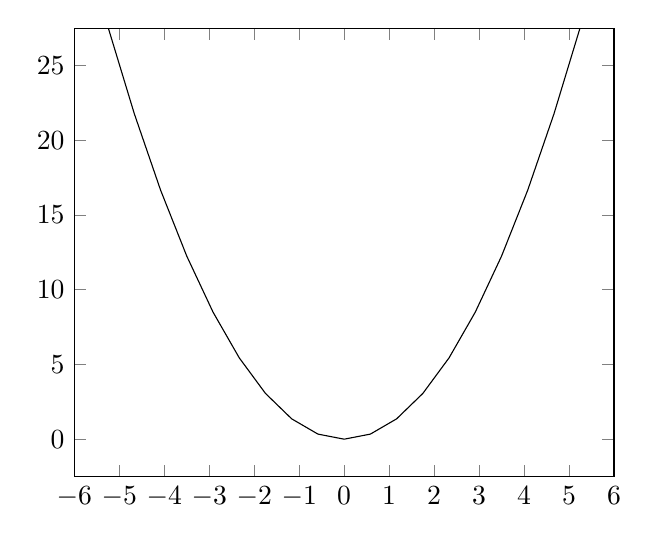
\begin{tikzpicture}
\begin{axis}[
xmin=-5,
xmax=5,
ymin=0,
ymax=25,
xtick distance=1,
ytick distance=5,
enlargelimits=true
]
\addplot[domain=-7:7] {x^2};
\end{axis}
\end{tikzpicture}

\vspace*{0.5cm}

\begin{tikzpicture}
\tkzTabInit{$x$ / 1, Variation de $f$ / 1.5}{$-\infty$, $+\infty$};
\end{tikzpicture}
\end{center}
\end{minipage}
\hfill
\begin{minipage}{0.4\textwidth}
\begin{center}
\textbf{Fonction racine carrée $\function{f}{[0;+\infty]}{\R}{x}{\sqrt{x}}$}
\begin{tikzpicture}
\begin{axis}[
xmin=0,
xmax=5,
ymin=0,
ymax=5,
xtick distance=1,
ytick distance=1,
enlargelimits=true
]
\addplot[domain=0:6] {sqrt(x)};
\end{axis}
\end{tikzpicture}

\vspace*{0.5cm}

\begin{tikzpicture}
\tkzTabInit{$x$ / 1, Variation de $f$ / 1.5}{$0$, $+\infty$};
\end{tikzpicture}
\end{center}
\end{minipage}

\vspace*{0.25cm}
\hrule
\vspace*{0.25cm}

\begin{minipage}{0.4\textwidth}
\begin{center}
\textbf{Fonction inverse\\$\function{f}{]-\infty;0[\cup]0;+\infty[}{\R}{x}{\dfrac{1}{x}}$}
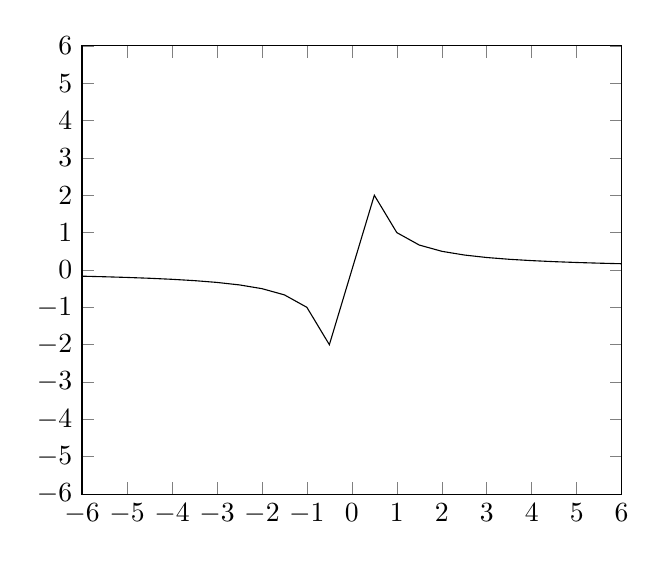
\begin{tikzpicture}
\begin{axis}[
xmin=-5,
xmax=5,
ymin=-5,
ymax=5,
xtick distance=1,
ytick distance=1,
enlargelimits=true
]
\addplot[domain=-6:6] {1/x};
\end{axis}
\end{tikzpicture}

\vspace*{0.5cm}

\begin{tikzpicture}
\tkzTabInit[espcl=1.75]{$x$ / 1, Variation de $f$ / 1.5}{$-\infty$,$0$, $+\infty$};
\tkzTabLine{ , ,d, , };
\end{tikzpicture}
\end{center}
\end{minipage}
\hfill
\begin{minipage}{0.4\textwidth}
\begin{center}
\textbf{Fonction cube\\$\function{f}{\R}{\R}{x}{x^3}$}
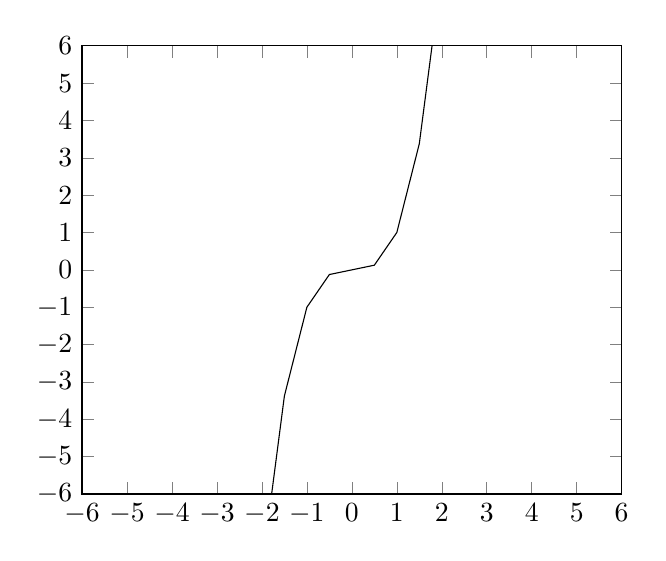
\begin{tikzpicture}
\begin{axis}[
xmin=-5,
xmax=5,
ymin=-5,
ymax=5,
xtick distance=1,
ytick distance=1,
enlargelimits=true
]
\addplot [domain=-6:6] {x^3};
\end{axis}
\end{tikzpicture}

\vspace*{0.5cm}

\begin{tikzpicture}
\tkzTabInit{$x$ / 1, Variation de $f$ / 1.5}{$-\infty$, $\infty$};
\end{tikzpicture}
\end{center}
\end{minipage}

\newpage
\subsection{Fonctions affines}
\begin{definition}
Une fonction affine est une fonction de la forme $x \mapsto ax + b$, définie sur $\R$, où $a$ est un nombre réel non nul (appelé \textbf{coefficient directeur}) et $b \in \R$ (appelé \textbf{ordonnée à l'origine}).
\end{definition}
\begin{remark}
\hfill
\begin{itemize}
\item Quand $b = 0$, on dit que la fonction est linéaire. 
\item La définition impose que $a$ soit différent de $0$, mais si c'est le cas, on dit que la fonction $x \mapsto b$ est une fonction constante.
\end{itemize}
\end{remark}
\begin{proposition}
\hfill
\begin{itemize}
\item Soit $f$ une fonction affine. Alors sa courbe représentative $\mathcal{C}_f$ est une droite.
\item Soit une fonction $f$ dont la courbe représentative $\mathcal{C}_f$ est une droite. Alors $f$ est une fonction affine.
\end{itemize}
\end{proposition}
\begin{example}
Soit $f$ une fonction dont la courbe représentative est donnée ci-dessous.
\begin{center}
\begin{tikzpicture}
\begin{axis}[width=8cm,xmin=-5,xmax=5,ymin=-5,ymax=5]
\addplot[domain=-6:6] {x - 4};
\end{axis}
\end{tikzpicture}
\end{center}
\begin{alphaquestions}
\item Justifier que $f$ est une fonction affine.
\item En déduire son expression algébrique.
\item Tracer la courbe représentative de la fonction $g : x \mapsto -2x -2$
\end{alphaquestions}
\end{example}
\begin{proposition}
Soit une fonction affine $f : x \mapsto ax + b$. Alors :
\begin{itemize}
\item $f$ est strictement croissante sur $\R$ si et seulement si $a > 0$; 
\item $f$ est strictement décroissante sur $\R$ si et seulement si $a < 0$ 
\end{itemize}
\end{proposition}
\begin{proposition}
Soit $f : x \mapsto ax + b$ une fonction affine, et $x_1 < x_2$ deux nombres réels. Alors, 
\begin{equation*}
a = \dfrac{f(x_2) - f(x_1)}{x_2 - x_1}
\end{equation*}
\end{proposition}

\newpage
\section{Tableaux de signe}
\subsection{Definition}

\begin{minipage}{0.45\textwidth}
\begin{center}
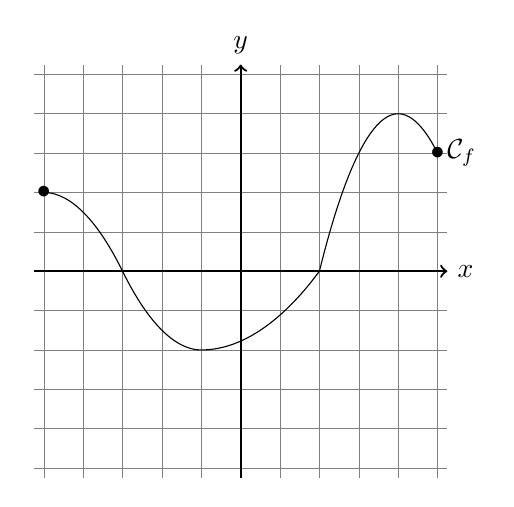
\begin{tikzpicture}[scale=0.5]
\draw[help lines] (-5.25,-5.25) grid (5.25,5.25);
\draw[->,thick] (-5.25,0) -- (5.25,0) node[right] {$x$}; 
\draw[->,thick] (0,-5.25) -- (0,5.25) node[above] {$y$};
\draw (-5,2) node {$\bullet$};
\draw (5,3) node {$\bullet$} node[right] {$\mathcal{C}_f$};
\draw (-5,2) parabola (-3,0);
\draw (-3,0) parabola[bend at end] (-1,-2);
\draw (-1,-2) parabola (2,0);
\draw (2,0) parabola bend (4,4) (5,3);
\end{tikzpicture}
\end{center}
\end{minipage}
\hfill\vline\hfill
\begin{minipage}{0.45\textwidth}
\begin{center}
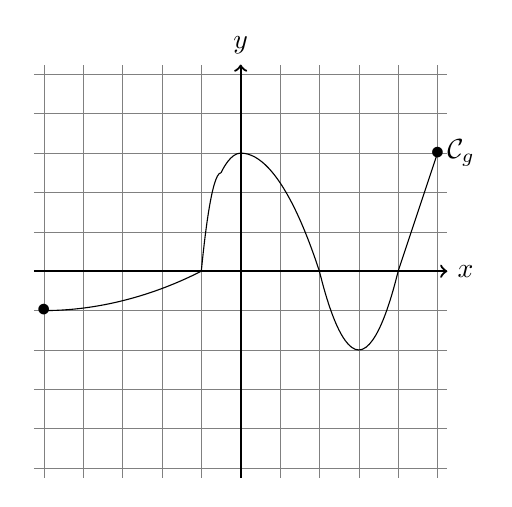
\begin{tikzpicture}[scale=0.5]
\draw[help lines] (-5.25,-5.25) grid (5.25,5.25);
\draw[->,thick] (-5.25,0) -- (5.25,0) node[right] {$x$}; 
\draw[->,thick] (0,-5.25) -- (0,5.25) node[above] {$y$};
\draw (-5,-1) node {$\bullet$};
\draw (5,3) node {$\bullet$} node[right] {$\mathcal{C}_g$};
\draw (-5,-1) parabola (-1,0);
\draw (-1,0) parabola[bend at end] (-0.5,2.5);
\draw (-0.5,2.5) parabola bend (0,3) (2,0);
\draw (2,0) parabola bend (3,-2) (4,0);
\draw (4,0) -- (5,3);
\end{tikzpicture}
\end{center}
\end{minipage}
\begin{definition}
Le tableau de signe d'une fonction $f$ répertorie les intervalles solutions de $f(x) \geq 0$ (où la fonction est \textbf{positive}) et $f(x) \leq 0$ (où la fonction est \textbf{négative}).
\end{definition}
\begin{example}
\hfill

\vspace*{0.2cm}
\begin{minipage}{0.45\textwidth}
\begin{tikzpicture}
\tkzTabInit[espcl=1.5]{$x$ / 1, Signe de $f$ / 2}{$-5$,$-3$,$2$,$5$};
\tkzTabLine{,+,z,-,z,+,};
\end{tikzpicture}
\end{minipage}
\hfill\vline\hfill
\begin{minipage}{0.45\textwidth}
\begin{tikzpicture}
\tkzTabInit[espcl=1.5]{$x$ / 1, Signe de $g$ / 2}{$-5$,,,$5$};
\tkzTabLine{,,,,,,};
\end{tikzpicture}
\end{minipage}
\end{example}

\subsection{Fonctions affines}

\begin{proposition}
Soit $f : x \mapsto ax + b$ une fonction affine définie sur $\R$. Alors son tableau de signe est donné par
\begin{center}
\begin{tikzpicture}
\tkzTabInit{$x$ / 1, Signe de $f$ / 2}{$-\infty$,$\dfrac{-b}{a}$,$+\infty$};
\tkzTabLine{,\text{Signe de }-a,z,\text{Signe de }a,};
\end{tikzpicture}
\end{center}
\end{proposition}
\begin{remark}
Pour se souvenir de cette proposition, on obtient $\dfrac{-b}{a}$ en résolvant l'équation $ax + b = 0$. Pour les signes, on se souvient que la monotonie de la fonction affine est donnée par $a$.
\begin{itemize}
\item Si $f$ est croissante, alors on part d'en bas pour aller en haut ($-$ puis $+$).
\item Si $f$ est décroissante, alors on part d'en haut pour aller en bas ($+$ puis $-$).
\end{itemize}
\end{remark}
\begin{example}
Dresser les tableaux de signe de $f : x \mapsto 3x - 12$ et $g : x \mapsto -3x + 12$.
\end{example}


\newpage
\subsection{Tableaux de signe d'une fonction produit ou quotient}
\begin{remark}
Si la fonction dont on étudie le signe est un produit ou quotient de sous-fonctions dont on connait le signe, alors on construit un tableau de signes à plusieurs lignes.
\end{remark}
\begin{example}
On cherche à étudier le signe de $f : x \mapsto (4x + 12)(-x + 2)$ sur $\R$. C'est le produit de $x \mapsto (4x + 2)$ et $x \mapsto (-x + 2)$.
\begin{center}
\begin{tikzpicture}
\tkzTabInit{$x$ / 1, Signe de $(4x+2)$ / 1.5, Signe de $(-x + 2)$ / 1.5, Signe de $f$ / 1.5}{$-\infty$,$-3$,$2$,$+\infty$};
\tkzTabLine{,-,z,,+,,};
\tkzTabLine{,,+,,z,-,};
\tkzTabLine{,-,z,+,z,-,};
\end{tikzpicture}
\end{center}
Faire de même avec $g : x \mapsto (-3x - 8)(-6x + 4)$.
\end{example}
\begin{example}
On cherche à étudier le signe de $g : x \mapsto \dfrac{4x + 12}{-x + 2}$. Ici, on a un quotient, le zéro du dénominateur devient une valeur interdite (double barre).
\begin{center}
\begin{tikzpicture}
\tkzTabInit{$x$ / 1, Signe de $(4x+2)$ / 1.5, Signe de $(-x + 2)$ / 1.5, Signe de $f$ / 1.5}{$-\infty$,$-3$,$2$,$+\infty$};
\tkzTabLine{,-,z,,+,,};
\tkzTabLine{,,+,,z,-,};
\tkzTabLine{,-,z,+,d,-,};
\end{tikzpicture}
\end{center}
Faire de même avec $g : x \mapsto \dfrac{-3x - 8}{-6x + 4}$.
\end{example}
\newpage
\section{Extremum de fonction}
\begin{definition}
Soit $f$ une fonction définie sur un intervalle $I$, et $b$ un nombre réel.
\begin{itemize}
\item On dit que $b$ est un \textbf{maximum de $f$ sur $I$}, si pout tout $x \in I$, on a $f(x) \leq b$; et qu'il existe $a \in I$ tel que $f(a) = b$. On dit alors que le maximum $b$ de $f$ sur $I$ est atteint en $a$.
\item On dit que $b$ est un \textbf{minimum de $f$ sur $I$}, si pout tout $x \in I$, on a $f(x) \geq b$; et qu'il existe $a \in I$ tel que $f(a) = b$. On dit alors que le minimum $b$ de $f$ sur $I$ est atteint en $a$.
\end{itemize}
\end{definition}
\begin{remark}
\hfill
\begin{itemize}
\item Le maximum d'une fonction sur $I$ est donc la plus grande image possible sur $I$, tandis que le minimum est la plus petite image possible sur $I$.
\item Il y a deux choses à vérifier pour que $b$ soit un extremum : d'abord que tous les $f(x)$ sont bien supérieurs ou inférieurs à $b$ ($f(x) \leq b$ ou $f(x) \geq b$ pour TOUT $x$ dans l'ensemble de définition), puis qu'il y a un antécédant $a$ pour $b$ ($f(a) = b$ et $a$ est bien dans l'ensemble de définition).
\end{itemize}
\end{remark}
\begin{example}
Soit une fonction $f$ dont la courbe représentative est donnée ci-après :
\begin{center}
\begin{tikzpicture}[scale=0.5]
\draw[help lines] (-5.25,-5.25) grid[step=0.5] (5.25,5.25);
\draw[axis] (-5.25,0) -- (5.25,0) node[right] {$x$};
\draw[axis] (0,-5.25) -- (0,5.25) node[above] {$y$};
\draw (1,0.1) -- (1,-0.1) node[below] {$1$};
\draw (0.1,1) -- (-0.1,1) node[left] {$1$};
\draw (-5,4) node {$\bullet$};
\draw (-5,4) parabola bend (-2.5,-3.5) (0,-1);
\draw (0,-1) parabola bend (2,3) (5,-0.5);
\draw (5,-0.5) node {$\bullet$};
\end{tikzpicture}
\end{center}
\begin{alphaquestions}
\item Compléter le tableau de variation de $f$.
\begin{center}
\begin{tikzpicture}
\tkzTabInit[espcl=1.5]{$x$ / 1, Variation de $f$ / 2}{, , ,};
\end{tikzpicture}
\end{center}
\item Déterminer le maximum de cette fonction ? En quelle valeur ce maximum est-il atteint ?

\item Déterminer le minimum de cette fonction ? En quelle valeur ce minimum est-il atteint ? 
\end{alphaquestions}
\end{example}
\end{document}